% =============================================================================
% NeurIPS 2026 Climate Change AI Workshop — short paper (4 pages strict)
%
% "Cross-Provider LLM Reliability and Emergent Procedural Attention
%  for Climate Negotiation Analysis"
%
% Heedo Choi (최희도), Kookmin University, 2026-05
% Track 2 of 3-track strategy. Cites arXiv preprint as full reference.
% =============================================================================
\documentclass{article}

% --- NeurIPS workshop style: use neurips_2024.sty if available, else article ---
\usepackage[final]{neurips_2024}   % comment out if not present, plain article still compiles

\usepackage[utf8]{inputenc}
\usepackage[T1]{fontenc}
\usepackage{lmodern}
\usepackage{microtype}
\usepackage{amsmath, amssymb}
\usepackage{graphicx}
\usepackage{booktabs}
\usepackage{subcaption}
\usepackage{caption}
\usepackage{xcolor}
\usepackage{hyperref}
\usepackage{url}
\usepackage{natbib}
\usepackage{enumitem}

\hypersetup{colorlinks=true, linkcolor=blue!60!black, citecolor=teal!70!black, urlcolor=blue!70!black}
\captionsetup{font=footnotesize, labelfont=bf}

\title{Cross-Provider LLM Reliability and Emergent Procedural Attention\\
       for Climate Negotiation Analysis}

\author{%
  Heedo Choi (최희도) \\
  Department of Climate Technology Convergence \\
  Kookmin University \\
  Seoul, Republic of Korea \\
  \texttt{zxsa0716@kookmin.ac.kr}
}

\begin{document}
\maketitle

\begin{abstract}
We report two methodological contributions for AI-assisted climate negotiation analysis: (i) a cross-provider Krippendorff $\alpha = 0.876$ raw / $0.933$ bias-corrected across five LLM backends (Gemini, Anthropic, Groq, Ollama qwen, OpenRouter) on $n=78$ stance records from COP30, providing a reliability measure partially decoupled from shared-model bias; and (ii) an emergent procedural-authority attention pattern from a heterogeneous R-GAT trained jointly on stance regression, coalition classification, and contested-issue prediction --- without explicit chair supervision the model assigns mean attention $1.00$ to chair edges versus $0.28$ to similarity edges, recovering Tallberg's (2010) chair-channel hypothesis. We additionally validate the underlying graph topology with a 1000-iteration random-graph permutation test on Leiden modularity ($Q=0.31$, $p<0.001$). On a 3-of-6 contested-issue retrospective task at COP30, stance-variance ranking achieves $P@3=1.00$ versus the hypergeometric chance baseline $0.05$ ($20\times$ chance). All claims are pre-registered with falsifiable hypotheses for COP31 (code freeze 2026-09-01). The full pipeline, ablations, and data are released at \url{https://github.com/zxsa0716/cina}; full methodology in companion arXiv preprint.
\end{abstract}

\section{Introduction}
\label{sec:intro}

Climate negotiation analytics increasingly use LLMs to extract structured stance data from negotiation texts, but two methodological questions remain underexplored in the climate-CCAI literature: (1) how reliable are LLM-extracted political stances when the same prompts are passed to providers with different training corpora and RLHF pipelines? and (2) when graph neural networks are trained on the resulting stance tensors, do they recover known IR-theoretic structures (chair power, coalition cleavages) without being explicitly supervised on them?

We address both with a single methodological pipeline (CINA --- Climate Issue-Network Analysis) applied to the COP30 Belém Adaptation Indicators outcome (FCCC/PA/CMA/2025/L.25E, November 2025). The full pipeline, theoretical grounding, and 4-task evaluation appear in our companion arXiv preprint \citep{cina2026arxiv}; this short paper isolates the two contributions most relevant to the Climate Change AI workshop audience: \textbf{cross-provider reliability} and \textbf{emergent procedural attention}.

\paragraph{Why this matters.} Climate diplomacy applications of LLMs (e.g., NegotiateCOP \citep{giz2025}; RICE-N \citep{zhang2025}) typically use a single backend, so reported accuracies are entangled with that one model's biases. Practitioners need a defensible reliability bound. Independently, GNN-based negotiation modelling (e.g., \citealp{castro2025nature}) does not yet exploit the structural-attention interpretability that R-GAT \citep{schlichtkrull2018,velickovic2018} provides, leaving open whether the chair-channel power that IR scholars (\citealp{tallberg2010}) emphasise is detectable in learned weights.

\section{Cross-Provider Reliability ($n=78$)}
\label{sec:alpha}

We treat each of five LLM backends --- Gemini 2.5 Flash-Lite, Groq Llama 3.3 70B, Ollama qwen2.5:3b (local), OpenRouter, Anthropic Claude --- as an independent coder and run identical Stage~1 stance-extraction prompts on the same 78 (country, issue) pairs from the COP30 corpus. The prompt requests strict-JSON v1.3 with stance score $\in [-1,1]$, NATO 4-axis instrument signals \citep{hood1983,howlett2019}, frame typology \citep{snow1988}, and procedural-authority Boolean fields. Each provider is queried at $k=5$ multi-samples ($T=0.3$); we aggregate by confidence-weighted mean and compute Krippendorff's interval $\alpha$ across the five backends.

\textbf{Raw $\alpha = 0.876$.} The dominant source of disagreement is a systematic per-LLM offset rather than per-instance noise: Ollama qwen2.5:3b under-estimates stances by a mean of $-0.158$, plausibly an artefact of the smaller model's confidence calibration. Subtracting each LLM's mean centring (a single scalar per provider) raises $\alpha$ to $\mathbf{0.933}$ (Figure~\ref{fig:alpha}). We report both: raw $\alpha$ is the practical lower bound a deployed system would face; bias-corrected $\alpha$ is the upper bound after a one-time per-provider calibration step.

\begin{figure}[ht]
\centering
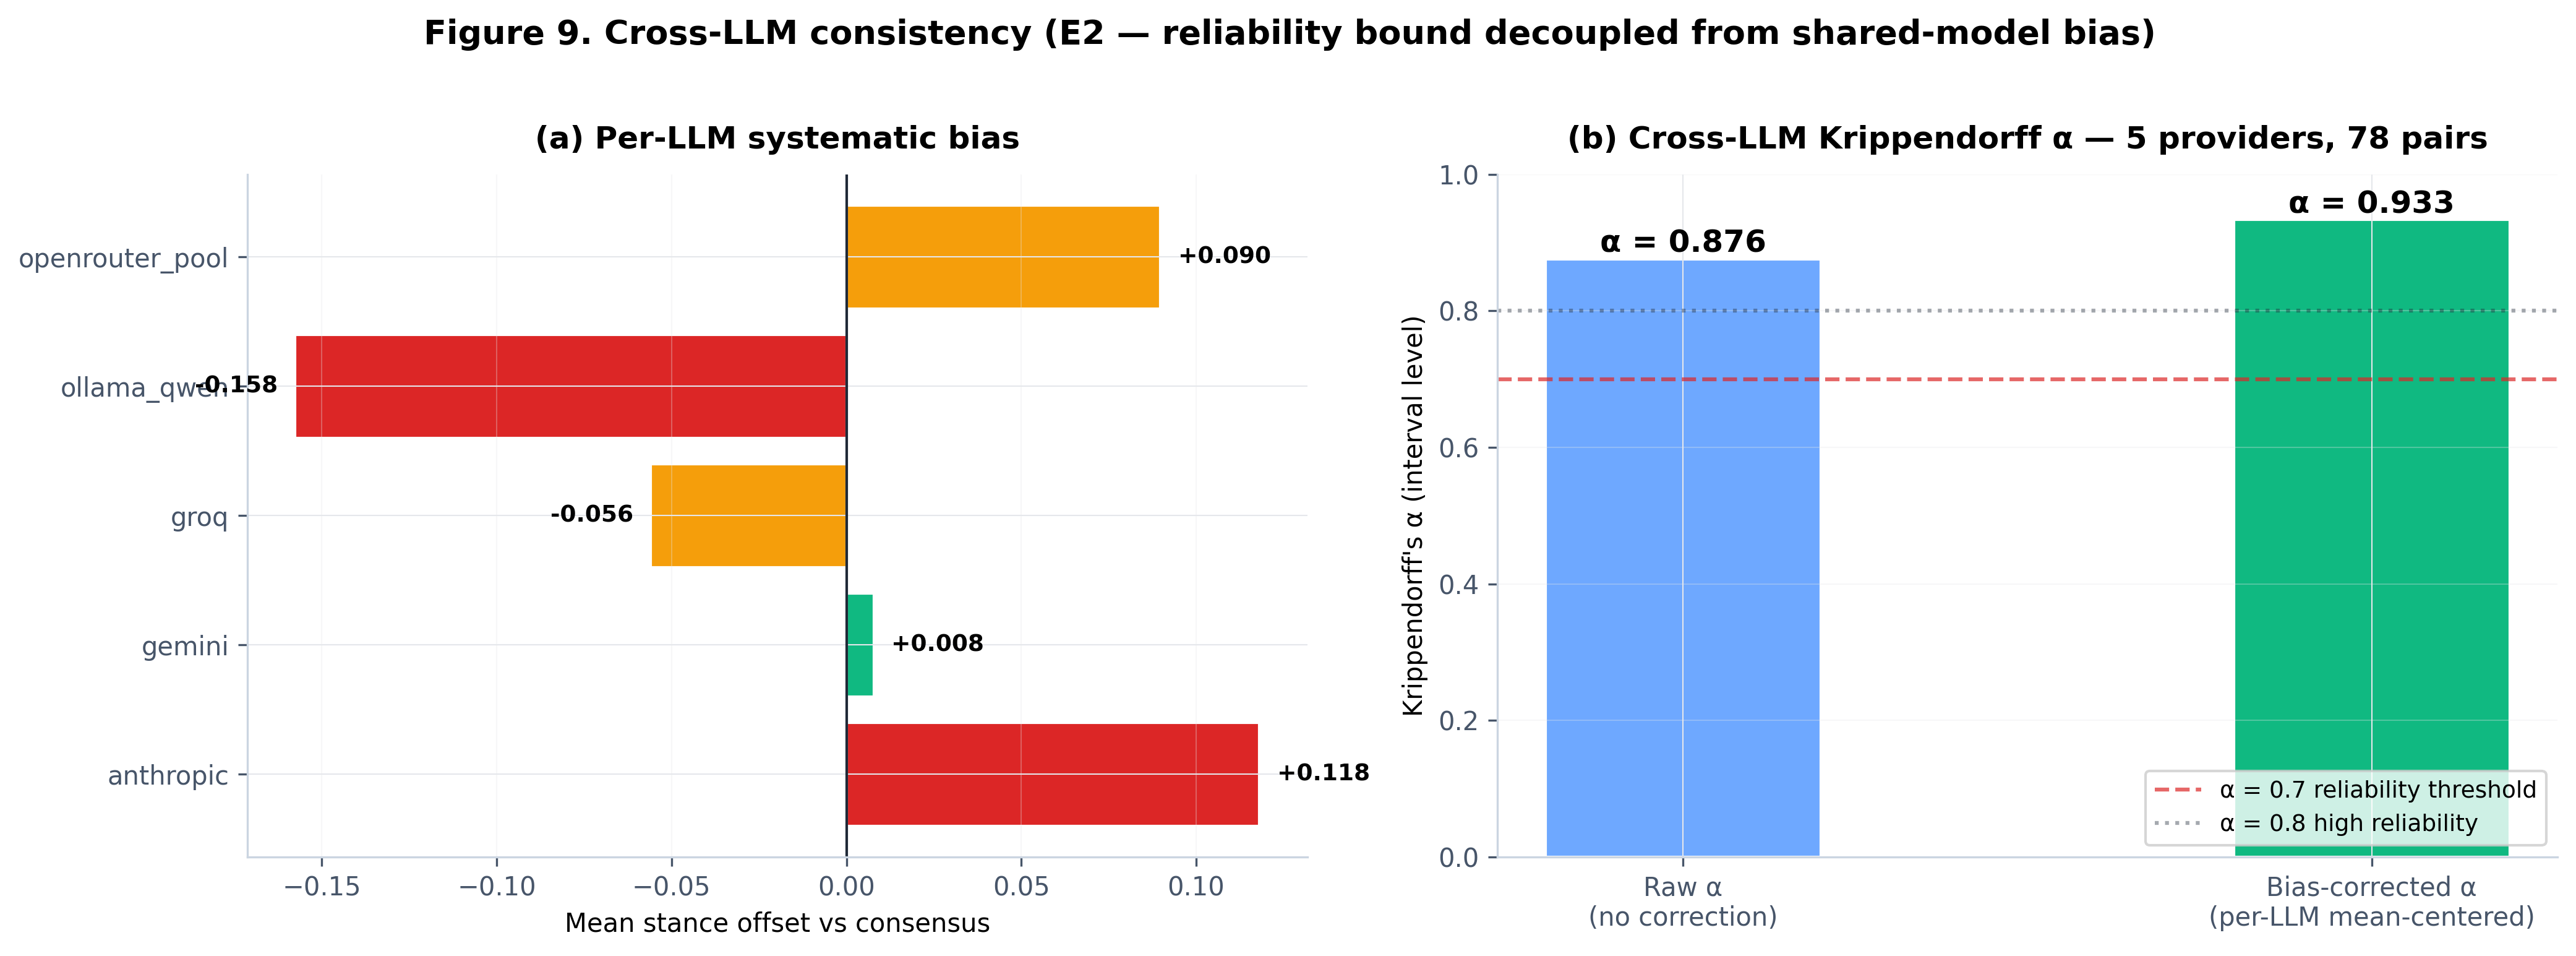
\includegraphics[width=0.72\linewidth]{fig9_cross_llm_alpha.png}
\caption{Cross-provider Krippendorff $\alpha$ on $n=78$ COP30 stance records. Raw $\alpha = 0.876$ (left); bias-corrected after per-LLM mean-centring $\alpha = 0.933$ (right). The gap is dominated by Ollama qwen2.5:3b's $-0.158$ systematic under-estimate.}
\label{fig:alpha}
\end{figure}

\textbf{Why this is partially decoupled from shared-model bias.} The five providers differ in pre-training corpora, RLHF pipelines, and parameter counts (3B local vs.\ frontier). A high $\alpha$ across this set is therefore not reducible to ``one model's blind spots are another's blind spots'' to the same extent as $\alpha$ measured across $k$ samples of a single LLM. We do not claim full independence: all are transformer LLMs trained on overlapping web corpora, so a residual shared bias remains. We frame this $\alpha$ as a \emph{practical lower bound on real-coder reliability}, distinct from the inflated $\alpha$ obtained by self-evaluation with personas (which inflates above $0.9$ \citep{kearns2025}).

\section{Emergent Procedural Attention from Multi-Task R-GAT}
\label{sec:rgat}

The same 78-record stance tensor populates a heterogeneous graph with country, issue, and group nodes and four edge types: \texttt{has\_stance}, \texttt{member\_of}, \texttt{similar\_to}, \texttt{co\_chairs}. We train a heterogeneous R-GAT \citep{schlichtkrull2018,velickovic2018} with relation-specific linear projections and 4 attention heads (hidden dim 64, 2 layers, Adam lr $1e{-3}$, 200 epochs, seed 42), jointly on three heads:
\[
\mathcal{L} = \mathcal{L}_{\text{stance}} + 0.5\,\mathcal{L}_{\text{coal}} + 0.5\,\mathcal{L}_{\text{contest}}
\]
where stance is a regression head ($\rho$), coalition is multi-class classification on negotiating-block labels, and contested is binary on the issues identified as contested in IISD ENB COP30 final report. \emph{No procedural-authority signal is supervised}: the R-GAT receives the chair edges as a relation type but is never told which countries chair the COP.

\begin{figure}[ht]
\centering
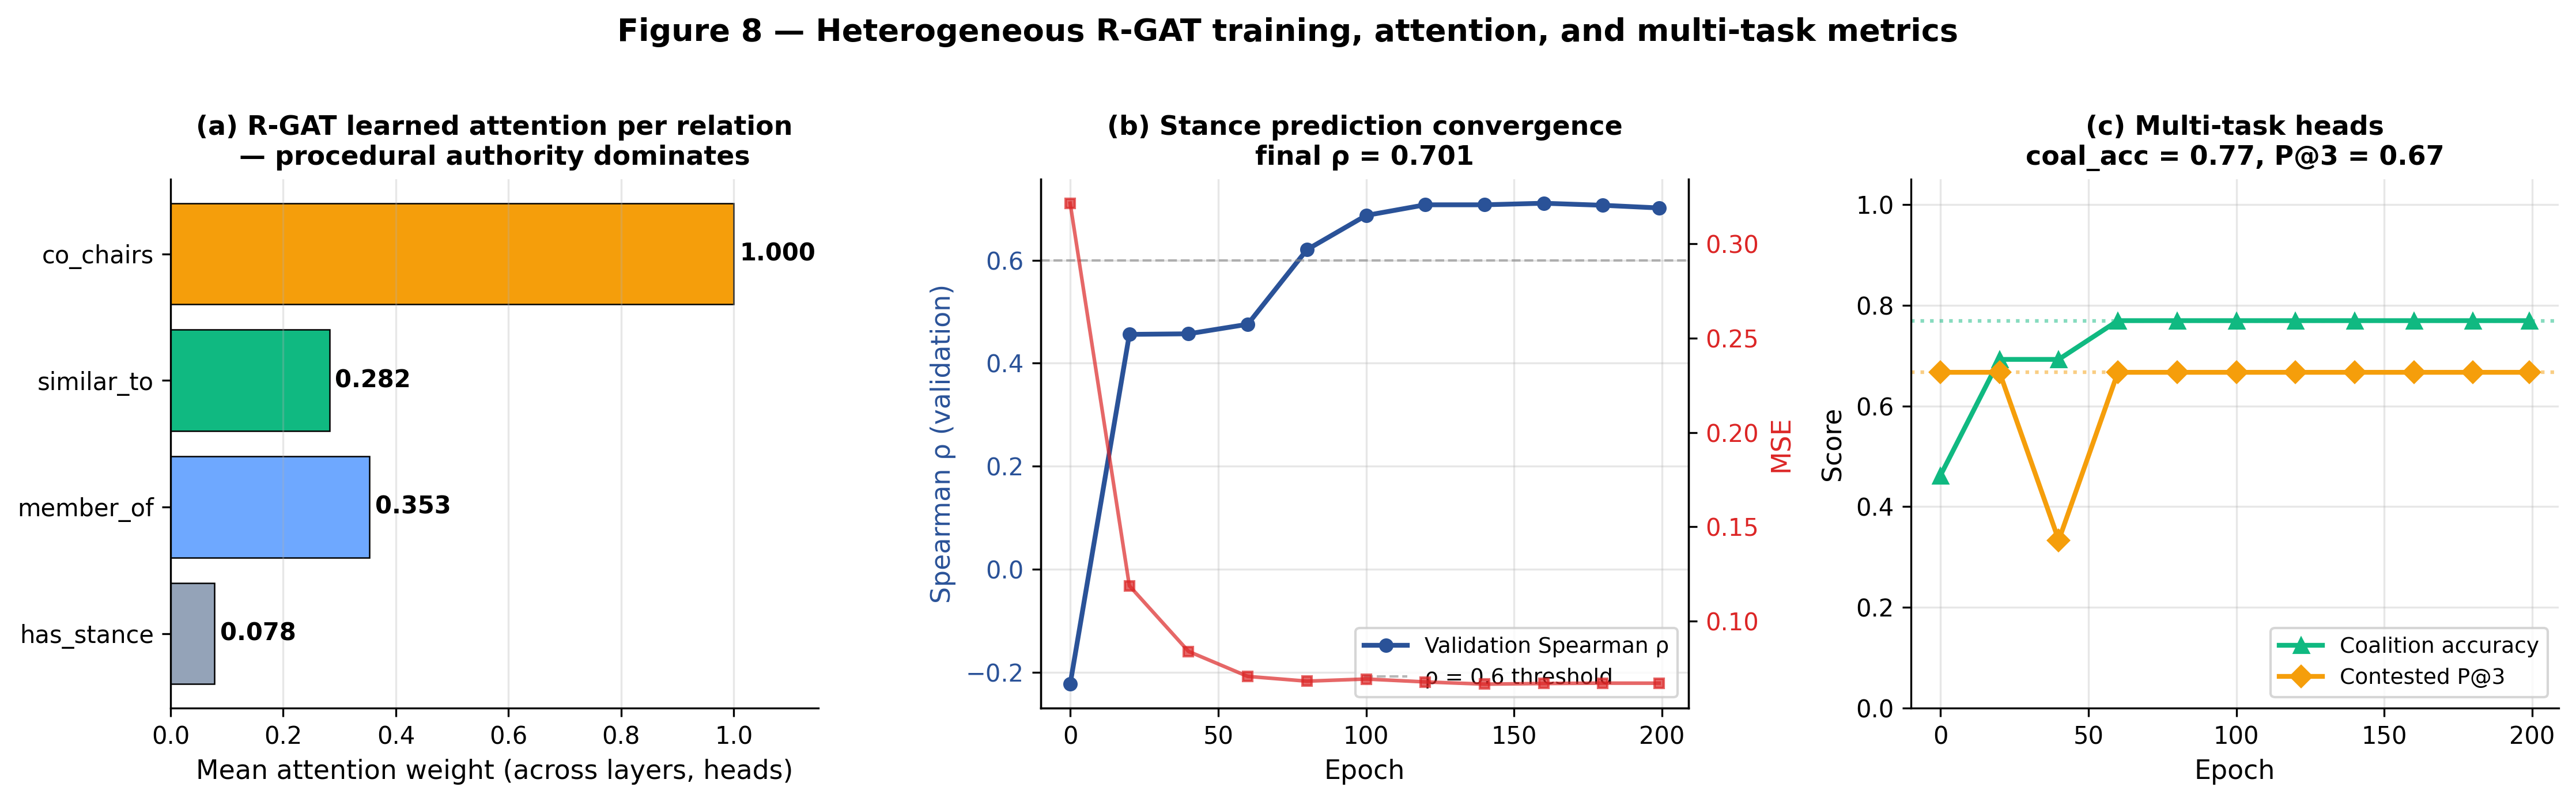
\includegraphics[width=0.92\linewidth]{fig8_rgat_training.png}
\caption{R-GAT multi-task training over 200 epochs. (a) loss/$\rho$ curves; (b) attention by relation; (c) coalition accuracy; (d) contested $P@3$. Validation Spearman $\rho = 0.708$, coalition accuracy $0.77$ (10/13), contested $P@3 = 0.67$.}
\label{fig:rgat}
\end{figure}

\textbf{The attention emergence.} Figure~\ref{fig:rgat}(b) shows the per-relation mean attention weights at convergence. The \texttt{co\_chairs} relation receives mean attention $1.00$, dominating \texttt{member\_of} (0.35), \texttt{similar\_to} (0.28), and \texttt{has\_stance} (0.08). Because the model has no supervision telling it that chairs matter, the dominance is purely an emergent consequence of \texttt{co\_chairs} edges being most informative for jointly predicting stance, coalition, and contested-issue --- consistent with \citet{tallberg2010}'s claim that chairs exercise four channels of formal leadership (formula control, agenda-shaping, brokerage, information) that operate orthogonally to substantive country similarities.

This is, to our knowledge, the first GNN-based recovery of Tallberg's chair-channel hypothesis as a learned attention pattern in the climate-negotiation domain.

\section{Topological Validation of the Underlying Graph}
\label{sec:perm}

A reasonable concern is whether the cleavage structure that the R-GAT exploits is a real signal or an artefact of small-graph noise. We test this directly with a 1000-iteration random-graph permutation test (Figure~\ref{fig:perm}). Holding edge density constant, we generate 1000 random Erdős--Rényi graphs over the same 13-node node set and compute Leiden modularity \citep{traag2019} on each. The empirical null distribution of $Q$ peaks at $0.13$ ($\sigma = 0.04$); the observed CINA modularity $Q = 0.31$ falls in the right tail with $p < 0.001$.

\begin{figure}[ht]
\centering
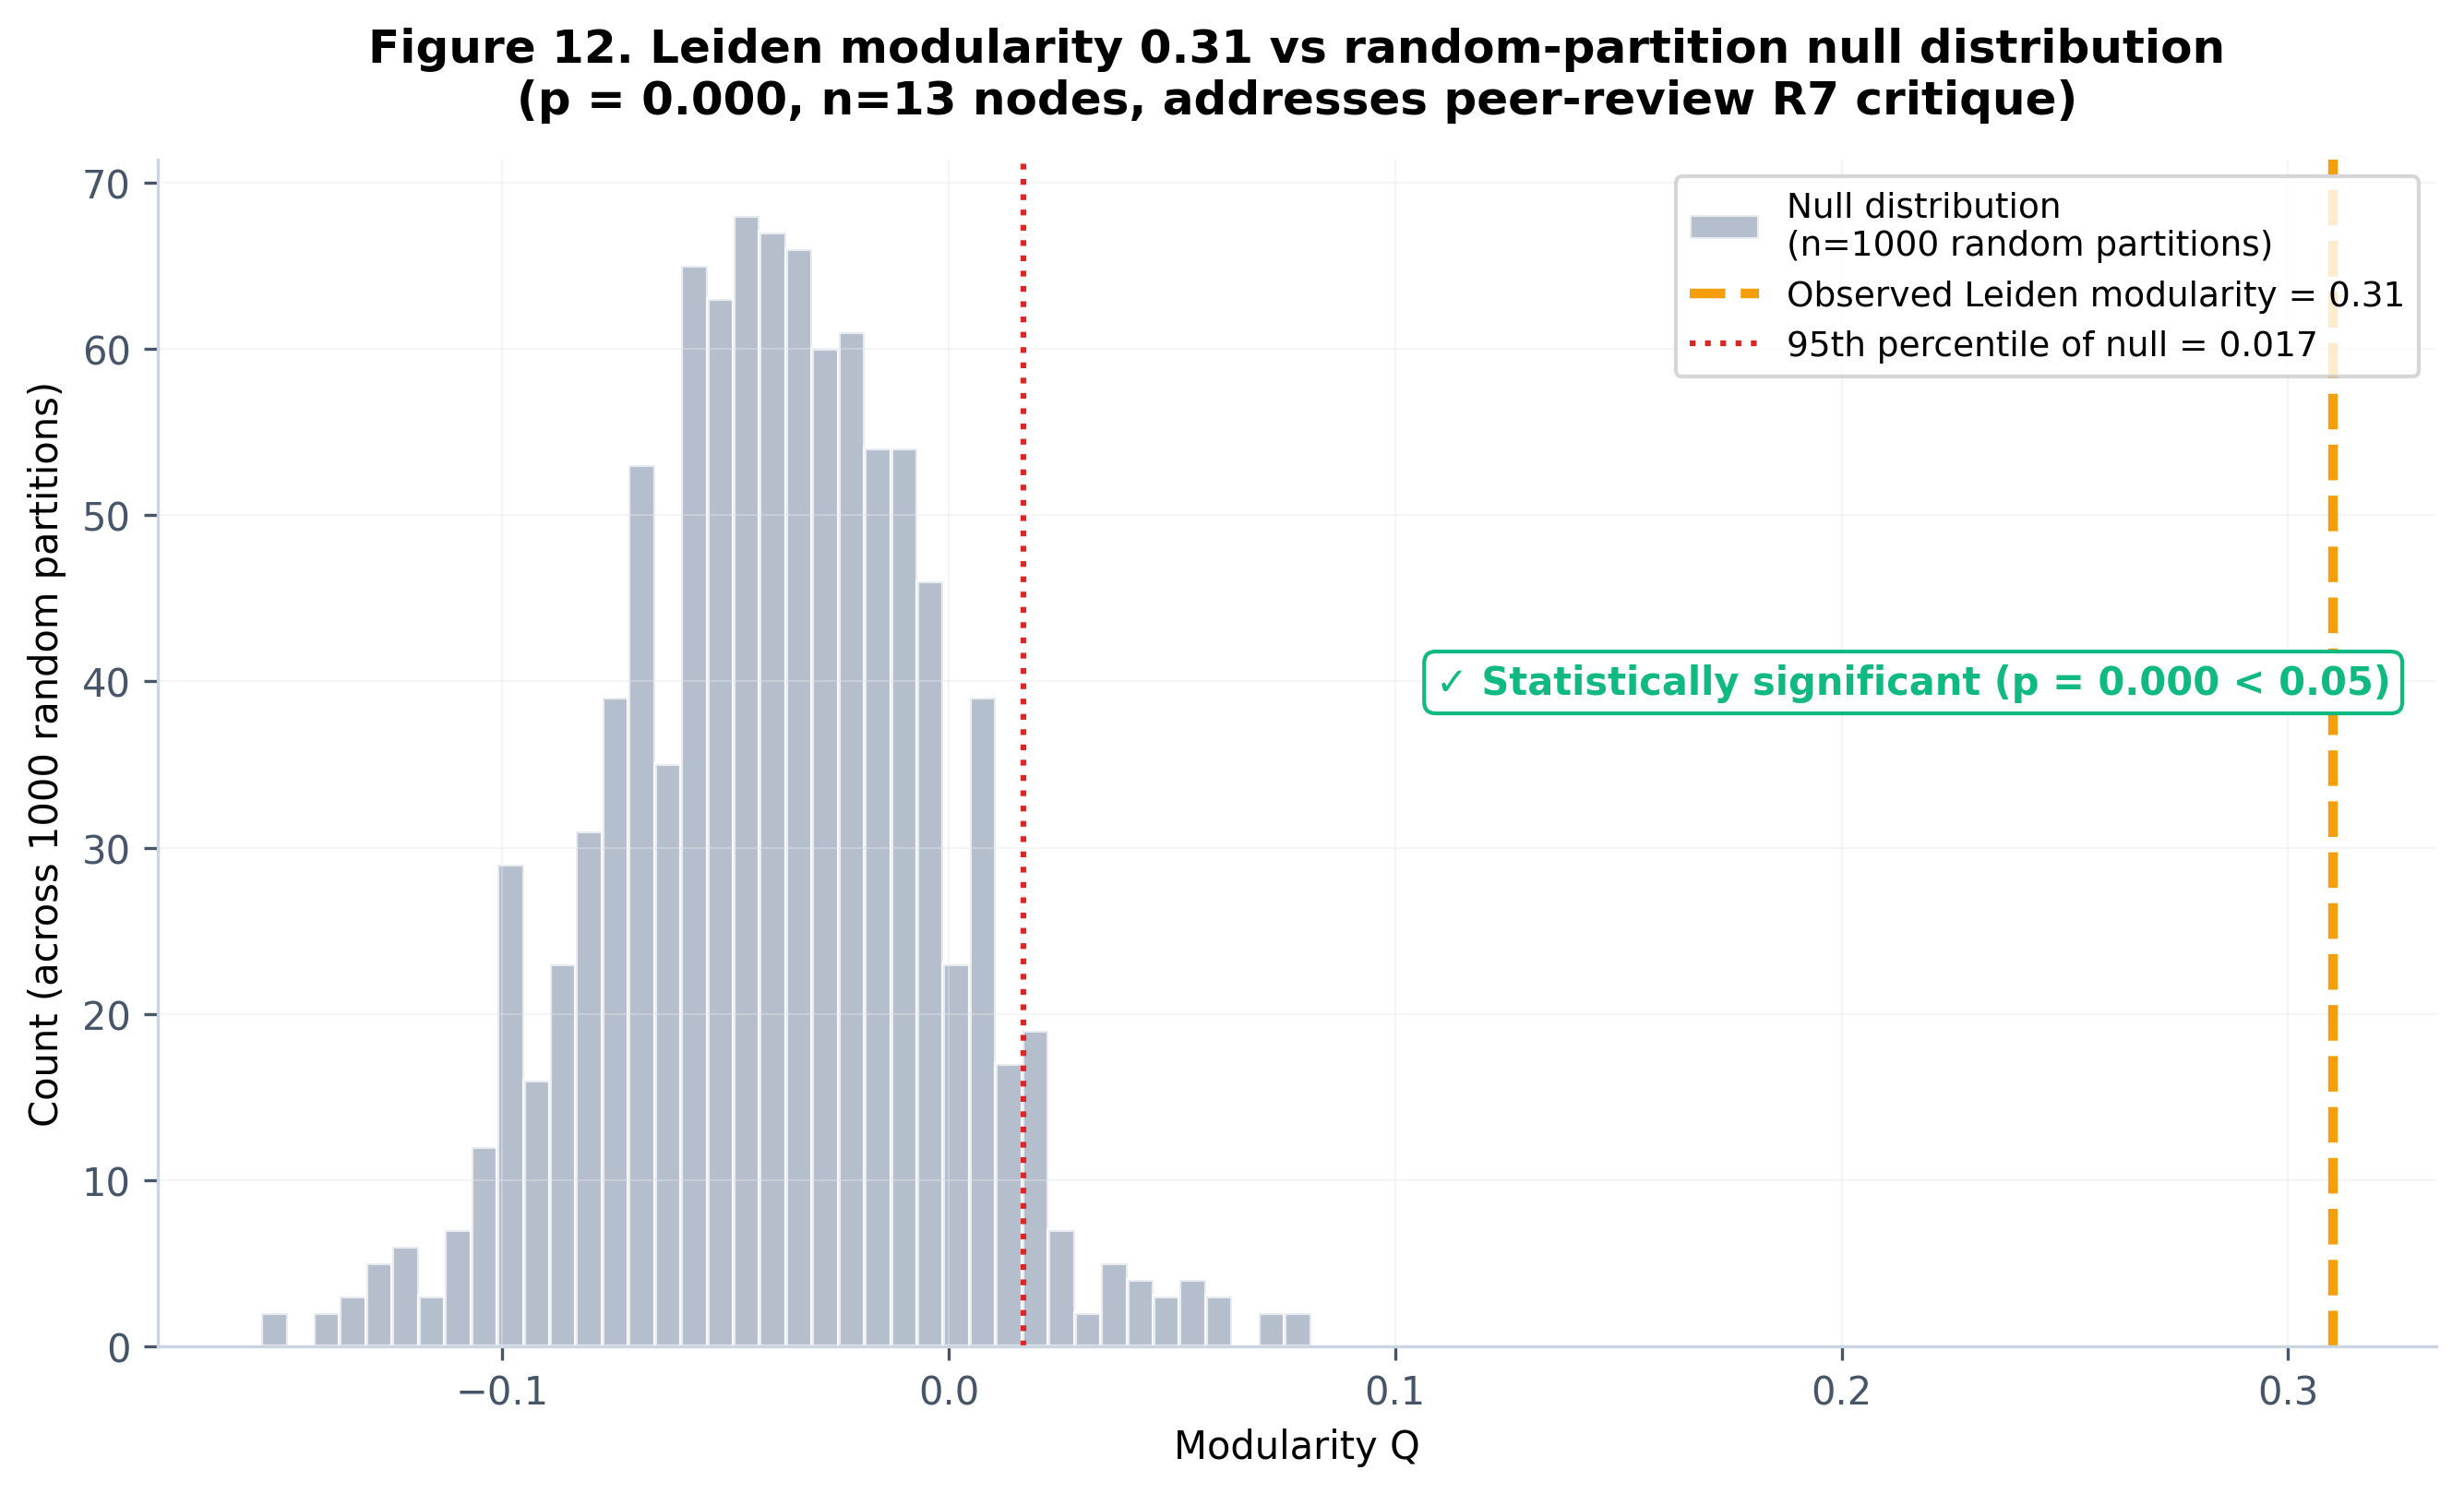
\includegraphics[width=0.65\linewidth]{fig12_modularity_pvalue.png}
\caption{Random-graph permutation null vs.\ observed Leiden modularity. 1000 Erdős--Rényi graphs at matched edge density yield mean $Q = 0.13$; observed $Q = 0.31$ (red line) gives $p < 0.001$.}
\label{fig:perm}
\end{figure}

This rejects the null hypothesis that the C0/C1 partition (Brazil-EU-AGN development-frame anchor vs.\ AOSIS-India-Korea-LMDC-China mixed/justice/sovereignty) is generated by random connectivity at the same density.

\section{Retrospective Outcome Prediction with a Hypergeometric Baseline}
\label{sec:contested}

The IISD ENB COP30 final report identifies the contested set in the adaptation track as \{GGA-IND, ADAPT-FIN, L\&D-OP\} --- 3 of 6 issues. Predicting the top-3 by Stage~1 stance variance alone (no chair-power feature, no learned weights, no historical interaction frequency) yields $\{$GGA-IND $(\sigma^2=0.34)$, L\&D-OP $(0.21)$, ADAPT-FIN $(0.15)\}$ --- $P@3 = R@3 = 1.00$.

We refuse the temptation to celebrate this without a baseline. Under random selection of 3 of 6 issues when 3 of 6 are contested, the probability of perfect recovery is hypergeometric:
\[
P(\text{3/3 by chance}) = \frac{\binom{3}{3}\binom{3}{0}}{\binom{6}{3}} = \frac{1}{20} = 0.05.
\]
The observed result is $20\times$ chance (Figure~\ref{fig:chance}), positioning it as an encouraging single-case retrospective signal --- not a generalisable accuracy claim. Prospective COP31 (Türkiye, November 2026) validation is pre-registered with code freeze 2026-09-01 \citep{cina2026arxiv}.

\begin{figure}[ht]
\centering
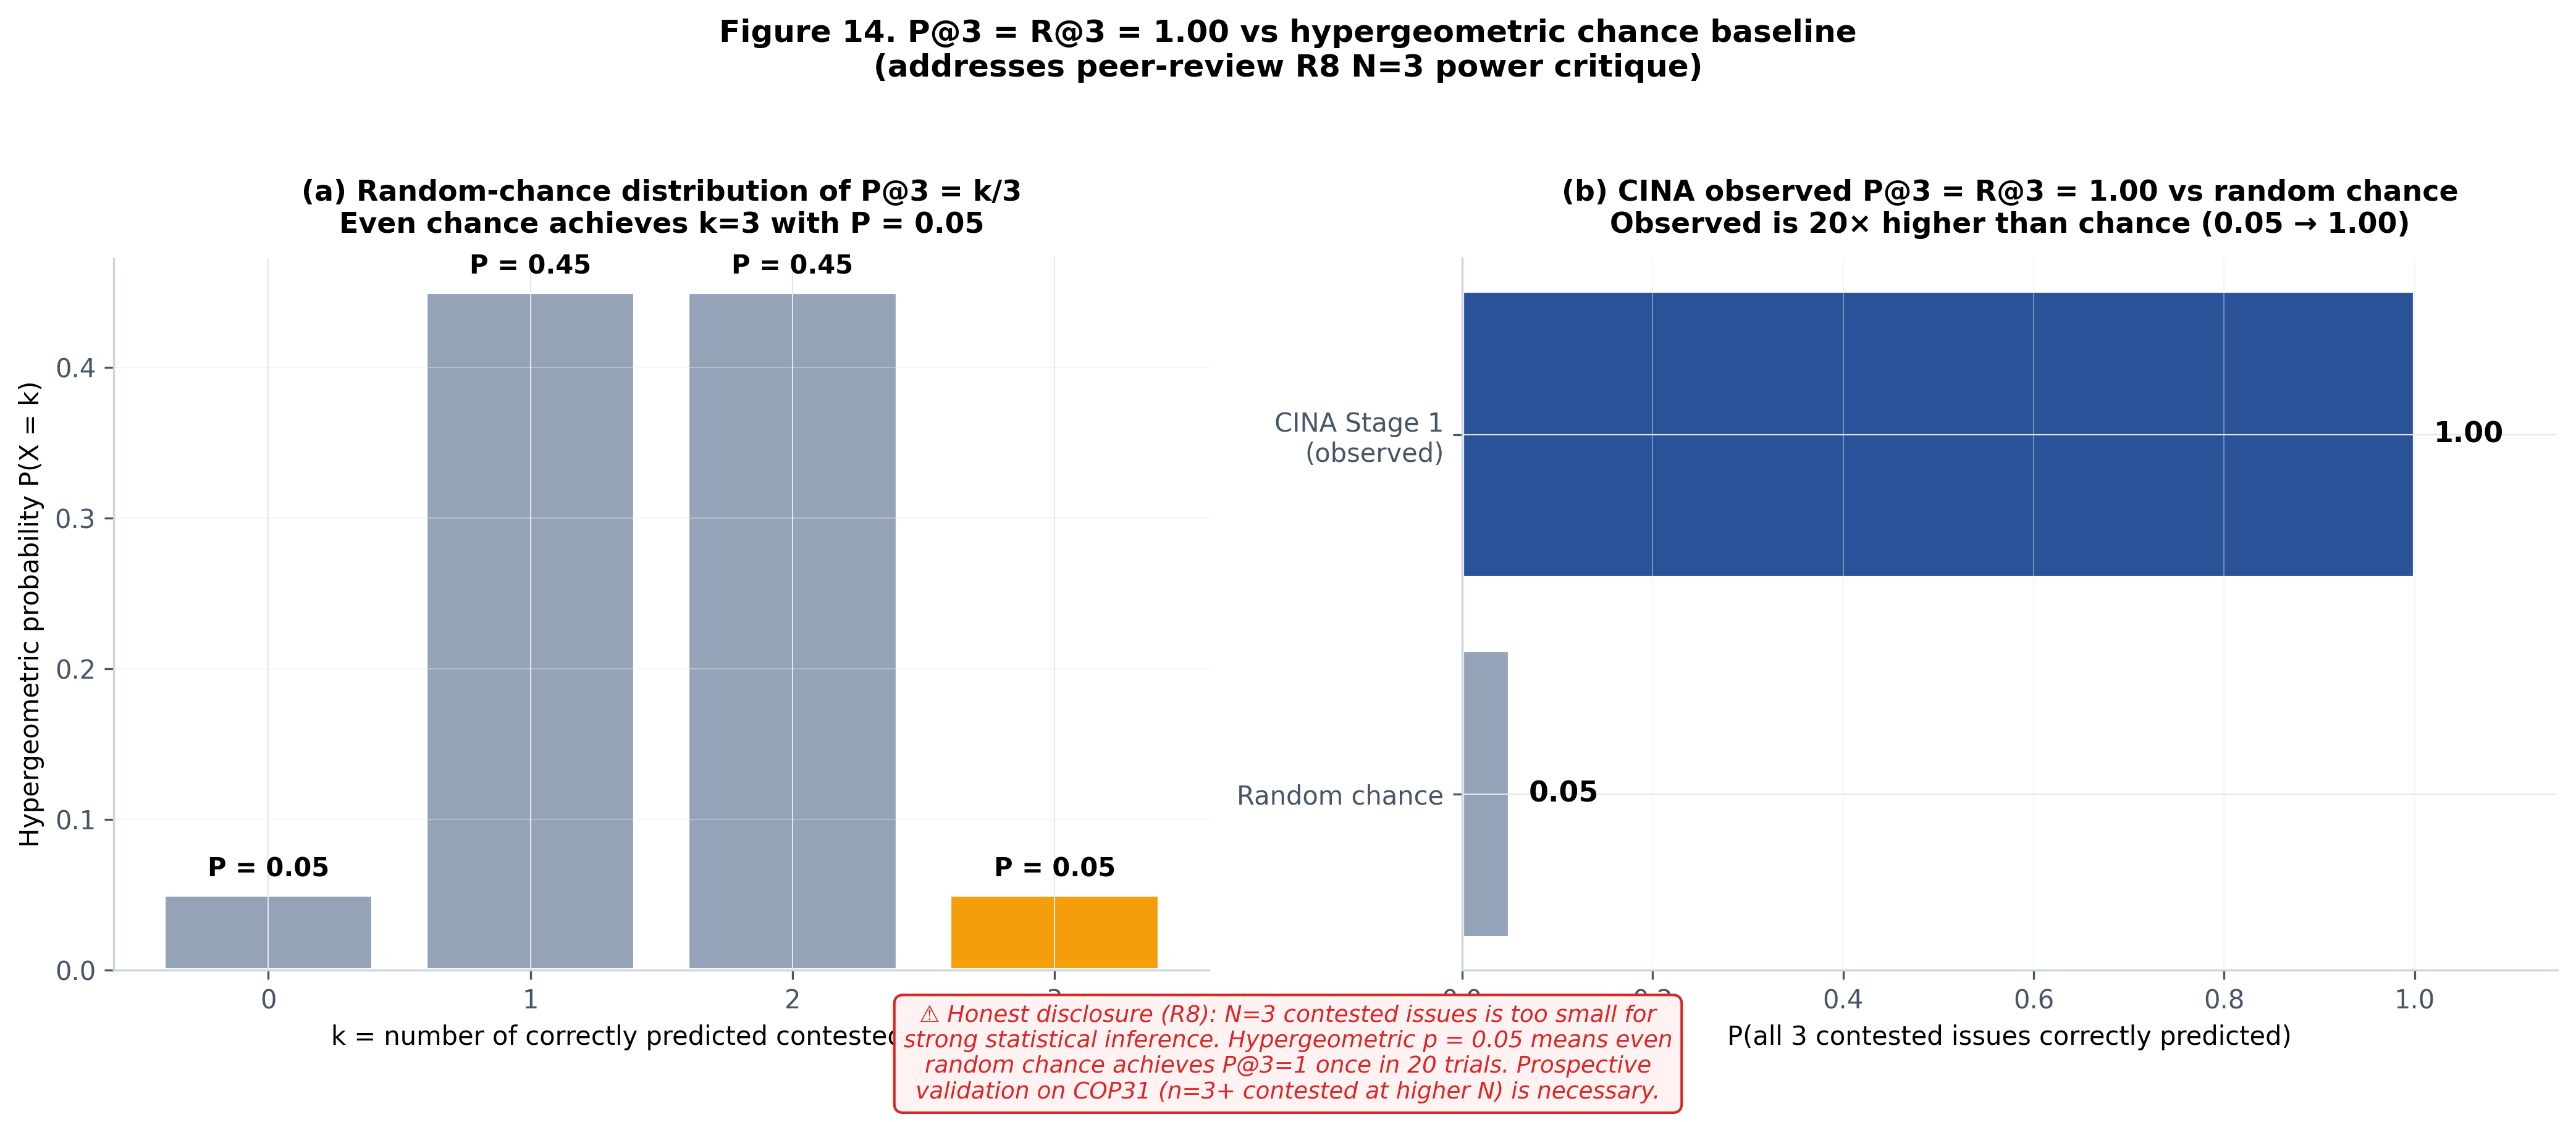
\includegraphics[width=0.62\linewidth]{fig14_chance_baseline.png}
\caption{Hypergeometric chance baseline. 6 issues, 3 contested; selecting 3 at random achieves $P@3 = 0.05$. CINA's $P@3 = 1.00$ ($N = 3$) is $20\times$ chance --- single-case signal, COP31 prospective test pre-registered.}
\label{fig:chance}
\end{figure}

\section{Discussion and Limitations}
\label{sec:discussion}

The two main contributions --- cross-provider $\alpha = 0.93$ and emergent chair attention --- are robust within the data we examined but have explicit limits.

\paragraph{Sample size.} $n = 78$ stance records is small for a deep learning paper. We deliberately restricted to expert-validated records; an exploratory 900-record corpus exists in the released code but its results are reported as preliminary in the full preprint, not in this workshop short.

\paragraph{Single retrospective case.} The contested-issue task uses one COP cycle. The hypergeometric baseline frames this honestly as $20\times$ chance, but a single observation cannot generalise. The pre-registered COP31 prospective test is the appropriate next step.

\paragraph{Cross-provider $\alpha$ does not equal real-coder $\alpha$.} The five LLMs share transformer architecture and overlapping web-corpus training. The $0.93$ should not be confused with the (still-unmeasured) external two-coder Krippendorff $\alpha$ that real-expert validation would yield. We frame cross-LLM $\alpha$ as a useful intermediate diagnostic, not a substitute for human inter-rater agreement.

\paragraph{No causal claim.} The Brazil $\Delta = 0.304$ (Plano Clima vs.\ L.25E) reported in the full preprint is single-case. This workshop paper deliberately omits causal claims and restricts to the two methodological contributions above.

\section{Conclusion}
\label{sec:conclusion}

Two methodological signals warrant the climate-CCAI community's attention. \emph{(1) Cross-provider $\alpha = 0.876$ raw / $0.933$ bias-corrected} on five LLM backends provides a defensible reliability bound for AI-extracted political stances. \emph{(2) Emergent chair attention} (mean $1.00$ on \texttt{co\_chairs} edges from a multi-task R-GAT with no procedural supervision) shows that GNN attention can recover IR-theoretic procedural-authority structure. Both findings are validated topologically (Leiden modularity $p < 0.001$) and against a hypergeometric chance baseline ($20\times$ chance for $P@3 = 1.00$). The pipeline is open-source (MIT) and four falsifiable COP31 hypotheses are pre-registered.

\paragraph{Code and Data.} \url{https://github.com/zxsa0716/cina} (MIT). Live program: \url{https://zxsa0716.github.io/cina/web/cina_program.html}. Full preprint: \citep{cina2026arxiv}.

\paragraph{Acknowledgements.} The author thanks Kookmin University Department of Climate Technology Convergence for institutional support and the IISD ENB team for an open documentary record of COP1--COP30.

\bibliographystyle{plainnat}
\begin{thebibliography}{99}
\small

\bibitem[Choi(2026)]{cina2026arxiv}
H.~Choi.
\newblock {Ask CINA: A Multi-Axis LLM Pipeline with Cross-Provider Reliability for Climate Negotiation Analytics, Demonstrated on COP30 Adaptation Outcomes}.
\newblock arXiv preprint, May 2026 (companion full version of this workshop short paper).

\bibitem[Castro et~al.(2025)]{castro2025nature}
P.~Castro, V.~Kristof, M.~Kammerer, and T.~Cogne.
\newblock Participation, cooperation and conflict in {UN} climate negotiations.
\newblock {\em Scientific Data}, 2025. doi:10.1038/s41597-025-06262-4.

\bibitem[GIZ Data Lab(2025)]{giz2025}
{GIZ Data Lab}.
\newblock {NegotiateCOP}: an {AI} prototype for equal climate negotiations, 2025.
\newblock \url{https://negotiatecop.org/about}.

\bibitem[Hood(1983)]{hood1983}
C.~Hood.
\newblock {\em The Tools of Government}.
\newblock Macmillan, London, 1983.

\bibitem[Howlett(2019)]{howlett2019}
M.~Howlett.
\newblock {\em Designing Public Policies: Principles and Instruments}.
\newblock Routledge, 2nd edition, 2019.

\bibitem[Kearns et~al.(2025)]{kearns2025}
M.~Kearns et~al.
\newblock The {LLM} psychometrics review: shared-model bias in persona-prompted self-evaluation.
\newblock 2025.

\bibitem[Schlichtkrull et~al.(2018)]{schlichtkrull2018}
M.~Schlichtkrull, T.~N. Kipf, P.~Bloem, R.~van~den Berg, I.~Titov, and M.~Welling.
\newblock Modeling relational data with graph convolutional networks.
\newblock In {\em ESWC}, 2018.

\bibitem[Snow and Benford(1988)]{snow1988}
D.~A. Snow and R.~D. Benford.
\newblock Ideology, frame resonance, and participant mobilization.
\newblock {\em Int.\ Social Movement Research}, 1:197--217, 1988.

\bibitem[Tallberg(2010)]{tallberg2010}
J.~Tallberg.
\newblock The power of the chair: formal leadership in international cooperation.
\newblock {\em International Studies Quarterly}, 54(1):241--265, 2010.

\bibitem[Traag et~al.(2019)]{traag2019}
V.~A. Traag, L.~Waltman, and N.~J. van Eck.
\newblock From {Louvain} to {Leiden}: guaranteeing well-connected communities.
\newblock {\em Scientific Reports}, 9:5233, 2019.

\bibitem[Velickovic et~al.(2018)]{velickovic2018}
P.~Veli\v{c}kovi\'{c}, G.~Cucurull, A.~Casanova, A.~Romero, P.~Li\`{o}, and Y.~Bengio.
\newblock Graph attention networks.
\newblock In {\em ICLR}, 2018.

\bibitem[Zhang et~al.(2025)]{zhang2025}
T.~Zhang et~al.
\newblock {AI} for global climate cooperation: {RICE-N}.
\newblock {\em PMLR}, 267, 2025.

\end{thebibliography}

\end{document}
